\section{Exercises on Minimum Spanning Trees Problems}

\paragraph{}
	GTC has been provided with 50 locations to connect in a certain country. These locations need
to be connected in such a way that any two of these locations are able to communicate
with each other. All the connections need not be direct. Due to high bandwidth
requirements, GTC will use high capacity cables for the connections, and wants to
know the costs of laying the cable under various circumstances. In Figure \ref{graph2-1} we
have schematically depicted the 50 locations and all possible direct connections. The
numbers attached to the connections in Figure \ref{graph2-1} refer to the distances (in 10 kilometer
units) between locations. The cost of the cable is \texteuro 5,000 per kilometer.

\begin{figure}[H]
	\centering
	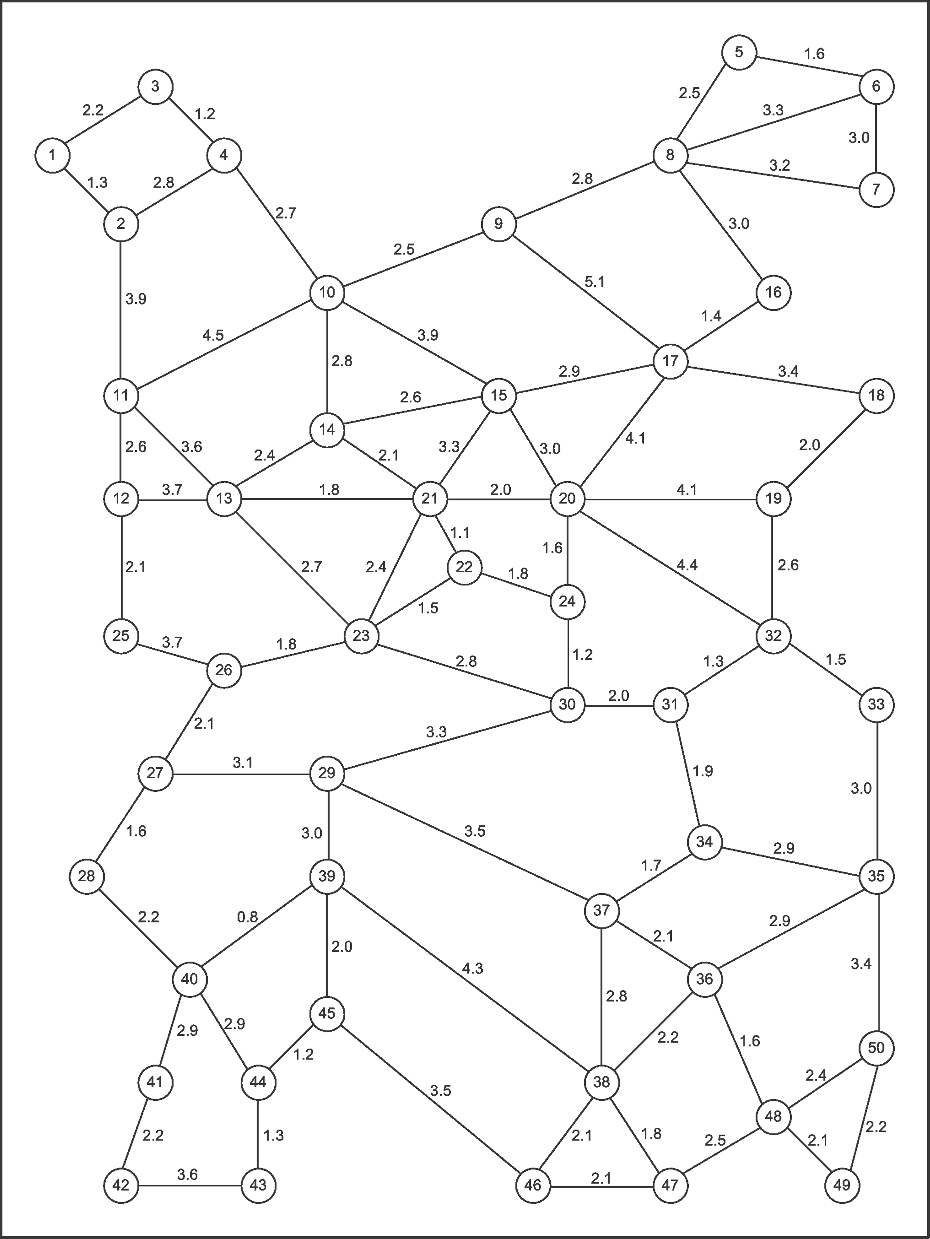
\includegraphics[scale=0.5]{./img/graph2-1.png}
	\caption{Schematic map with 50 locations (distances in 10 kilometer units, costs in \texteuro5,000per kilometer)}
	\label{graph2-1}
\end{figure}

\subsection{Problem 2.1. Reliable Cable Connections}
\begin{enumerate}[(a)]
\item \emph{Calculate the minimum length of cable needed to connect all locations in Figure
\ref{graph2-1}. Also give the list of connections that are used for the cabling.}
\end{enumerate}

\paragraph{}
	